% id: 57-17
% book: 100발100중 3-2 중간 · 01 3-2 중간(삼각비·삼각비의 활용·원과 직선·원주각·부록)
% section: 기출 Best 쌍둥이
% figure: crop:fig-57-17.png
% answer: ④
% answer_source: 답지(빠른정답)
% variant_level: 0 (원본 전사)
% 이 파일은 build.mjs 가 items.json 에서 만든다. 고칠 때는 items.json 을 고친다.
\smash{\raisebox{1.5mm}{\dmkichul{100발100중 3-2 중간 57쪽 17번}}}
\noindent\begin{minipage}[t]{0.58\linewidth}\vspace{0pt}\raggedright 그림에서 원~$\pt{O}$는 직사각형~$\pt{ABCD}$의 세 변과 접하고 $\seg{CE}$는 원~$\pt{O}$의 접선이다. $\seg{AB}=6\mkern3mu \mathrm{cm}$, $\seg{BC}=7\mkern3mu \mathrm{cm}$일 때, $\seg{CE}$의 길이는?\end{minipage}\hfill\begin{minipage}[t]{0.4\linewidth}\vspace{0pt}\centering 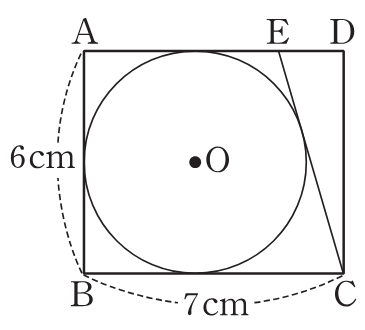
\includegraphics[width=87.5pt]{figures/fig-57-17.png}\end{minipage}\par
\begin{choices32}{\rule[-3ex]{0pt}{8ex}$\dfrac{7}{4}\mkern3mu \mathrm{cm}$}{\rule[-3ex]{0pt}{8ex}$\dfrac{15}{4}\mkern3mu \mathrm{cm}$}{\rule[-3ex]{0pt}{8ex}$\dfrac{21}{4}\mkern3mu \mathrm{cm}$}{\rule[-3ex]{0pt}{8ex}$\dfrac{25}{4}\mkern3mu \mathrm{cm}$}{\rule[-3ex]{0pt}{8ex}$8\mkern3mu \mathrm{cm}$}\end{choices32}
